\documentclass[aspectratio=169]{beamer}

\usepackage[utf8]{inputenc}
\usepackage{lmodern}
\usepackage[T1]{fontenc}
\usepackage{amsmath}
\usepackage{listings}
\usepackage{xcolor}
\usepackage{graphicx}
\usepackage{tikz}
\usetikzlibrary{arrows.meta, positioning, shapes.geometric, calc, graphs, quotes}

\makeatletter
\def\input@path{{../BeamerTemplate/theme/}}
\makeatother

\usetheme{CleanEasy}

\input{../BeamerTemplate/configs/configs}

\title{Graphs}
\subtitle{Modeling Relationships and Connectivity}
\author{Minseok Jeon}
\institute{DGIST}
\date{\today}

\begin{document}

\begin{frame}
  \titlepage
\end{frame}

\begin{frame}{Outline}
  \tableofcontents
\end{frame}

\section{Introduction to Graphs}

\begin{frame}{What is a Graph?}
  \textbf{Definition:} A collection of \textbf{nodes (vertices)} connected by \textbf{edges}.

  \vspace{0.3cm}
  \textbf{Formal notation:} G = (V, E)
  \begin{itemize}
    \item V = Set of vertices
    \item E = Set of edges (pairs of vertices)
  \end{itemize}

  \vspace{0.3cm}
  \begin{columns}[T]
    \begin{column}{0.5\textwidth}
      \textbf{Example Graph:}
      \begin{center}
        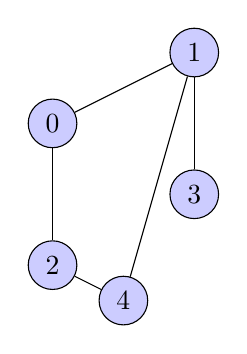
\begin{tikzpicture}[scale=0.9]
          \node[circle, draw, fill=blue!20] (0) at (0,1) {0};
          \node[circle, draw, fill=blue!20] (1) at (2,2) {1};
          \node[circle, draw, fill=blue!20] (2) at (0,-1) {2};
          \node[circle, draw, fill=blue!20] (3) at (2,0) {3};
          \node[circle, draw, fill=blue!20] (4) at (1,-1.5) {4};

          \draw (0) -- (1);
          \draw (0) -- (2);
          \draw (1) -- (3);
          \draw (1) -- (4);
          \draw (2) -- (4);
        \end{tikzpicture}
      \end{center}
    \end{column}

    \begin{column}{0.5\textwidth}
      \textbf{Components:}
      \begin{itemize}
        \item V = \{0, 1, 2, 3, 4\}
        \item E = \{(0,1), (0,2), (1,3), (1,4), (2,4)\}
        \item |V| = 5 vertices
        \item |E| = 5 edges
      \end{itemize}
    \end{column}
  \end{columns}
\end{frame}

\begin{frame}{Why Use Graphs?}
  \textbf{Graphs model relationships between entities:}

  \vspace{0.3cm}
  \begin{itemize}
    \item \textbf{Social networks:} People connected by friendships
    \item \textbf{Maps:} Cities connected by roads
    \item \textbf{Internet:} Websites connected by hyperlinks
    \item \textbf{Dependencies:} Tasks connected by prerequisites
    \item \textbf{Molecules:} Atoms connected by bonds
    \item \textbf{Recommendations:} Users/items connected by preferences
  \end{itemize}

  \vspace{0.3cm}
  \textbf{Fundamental questions:}
  \begin{itemize}
    \item Is there a path from A to B?
    \item What's the shortest path?
    \item Are all nodes connected?
    \item Does the graph contain cycles?
  \end{itemize}
\end{frame}

\section{Graph Representations}

\begin{frame}{Adjacency List Representation}
  \textbf{Idea:} Store a list of neighbors for each vertex.

  \vspace{0.3cm}
  \begin{columns}[T]
    \begin{column}{0.45\textwidth}
      \begin{center}
        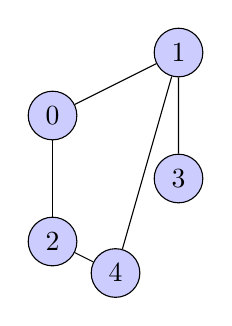
\begin{tikzpicture}[scale=0.8]
          \node[circle, draw, fill=blue!20] (0) at (0,1) {0};
          \node[circle, draw, fill=blue!20] (1) at (2,2) {1};
          \node[circle, draw, fill=blue!20] (2) at (0,-1) {2};
          \node[circle, draw, fill=blue!20] (3) at (2,0) {3};
          \node[circle, draw, fill=blue!20] (4) at (1,-1.5) {4};

          \draw (0) -- (1);
          \draw (0) -- (2);
          \draw (1) -- (3);
          \draw (1) -- (4);
          \draw (2) -- (4);
        \end{tikzpicture}
      \end{center}
    \end{column}

    \begin{column}{0.55\textwidth}
      \textbf{Adjacency List:}
      \begin{itemize}
        \item 0: [1, 2]
        \item 1: [0, 3, 4]
        \item 2: [0, 4]
        \item 3: [1]
        \item 4: [1, 2]
      \end{itemize}
    \end{column}
  \end{columns}

  \vspace{0.3cm}
  \textbf{Properties:}
  \begin{itemize}
    \item \textbf{Space:} O(V + E)
    \item \textbf{Add edge:} O(1)
    \item \textbf{Check edge:} O(degree)
    \item \textbf{Best for:} Sparse graphs (E $\ll$ V$^2$)
  \end{itemize}
\end{frame}

\begin{frame}[fragile]{Adjacency List Implementation}
  \begin{lstlisting}[language=Python, basicstyle=\ttfamily\small]
# Using dictionary
graph = {
    0: [1, 2],
    1: [0, 3, 4],
    2: [0, 4],
    3: [1],
    4: [1, 2]
}

# Using list of lists
graph = [
    [1, 2],      # neighbors of vertex 0
    [0, 3, 4],   # neighbors of vertex 1
    [0, 4],      # neighbors of vertex 2
    [1],         # neighbors of vertex 3
    [1, 2]       # neighbors of vertex 4
]

# With weights (weighted graph)
graph = {
    0: [(1, 5), (2, 3)],  # (neighbor, weight)
    1: [(0, 5), (3, 2), (4, 1)],
    2: [(0, 3), (4, 4)],
    3: [(1, 2)],
    4: [(1, 1), (2, 4)]
}
  \end{lstlisting}
\end{frame}

\begin{frame}{Adjacency Matrix Representation}
  \textbf{Idea:} 2D array where matrix[i][j] = 1 if edge (i,j) exists.

  \vspace{0.3cm}
  \begin{columns}[T]
    \begin{column}{0.45\textwidth}
      \begin{center}
        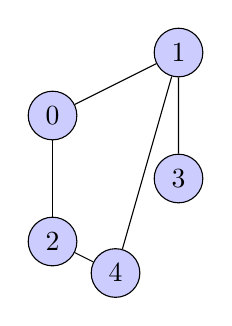
\begin{tikzpicture}[scale=0.8]
          \node[circle, draw, fill=blue!20] (0) at (0,1) {0};
          \node[circle, draw, fill=blue!20] (1) at (2,2) {1};
          \node[circle, draw, fill=blue!20] (2) at (0,-1) {2};
          \node[circle, draw, fill=blue!20] (3) at (2,0) {3};
          \node[circle, draw, fill=blue!20] (4) at (1,-1.5) {4};

          \draw (0) -- (1);
          \draw (0) -- (2);
          \draw (1) -- (3);
          \draw (1) -- (4);
          \draw (2) -- (4);
        \end{tikzpicture}
      \end{center}
    \end{column}

    \begin{column}{0.55\textwidth}
      \textbf{Adjacency Matrix:}
      \begin{center}
        \small
        \begin{tabular}{c|ccccc}
          & 0 & 1 & 2 & 3 & 4 \\
          \hline
          0 & 0 & 1 & 1 & 0 & 0 \\
          1 & 1 & 0 & 0 & 1 & 1 \\
          2 & 1 & 0 & 0 & 0 & 1 \\
          3 & 0 & 1 & 0 & 0 & 0 \\
          4 & 0 & 1 & 1 & 0 & 0 \\
        \end{tabular}
      \end{center}
    \end{column}
  \end{columns}

  \vspace{0.3cm}
  \textbf{Properties:}
  \begin{itemize}
    \item \textbf{Space:} O(V$^2$)
    \item \textbf{Add/check edge:} O(1)
    \item \textbf{Get neighbors:} O(V)
    \item \textbf{Best for:} Dense graphs (E $\approx$ V$^2$)
  \end{itemize}
\end{frame}

\begin{frame}[fragile]{Adjacency Matrix Implementation}
  \begin{lstlisting}[language=Python, basicstyle=\ttfamily\small]
# Unweighted graph (0 = no edge, 1 = edge)
n = 5
matrix = [
    [0, 1, 1, 0, 0],
    [1, 0, 0, 1, 1],
    [1, 0, 0, 0, 1],
    [0, 1, 0, 0, 0],
    [0, 1, 1, 0, 0]
]

# Weighted graph (0 or inf = no edge, value = weight)
inf = float('inf')
matrix = [
    [0,   5,   3,   inf, inf],
    [5,   0,   inf, 2,   1],
    [3,   inf, 0,   inf, 4],
    [inf, 2,   inf, 0,   inf],
    [inf, 1,   4,   inf, 0]
]

# Check if edge exists
def has_edge(matrix, u, v):
    return matrix[u][v] != 0  # or != inf for weighted

# Get all neighbors
def get_neighbors(matrix, u):
    return [v for v in range(len(matrix)) if matrix[u][v] != 0]
  \end{lstlisting}
\end{frame}

\begin{frame}{Comparison: List vs Matrix}
  \begin{table}
    \centering
    \begin{tabular}{|l|c|c|}
      \hline
      \textbf{Operation} & \textbf{Adjacency List} & \textbf{Adjacency Matrix} \\
      \hline
      Space & O(V + E) & O(V$^2$) \\
      \hline
      Add edge & O(1) & O(1) \\
      \hline
      Remove edge & O(degree) & O(1) \\
      \hline
      Check edge & O(degree) & O(1) \\
      \hline
      Get neighbors & O(degree) & O(V) \\
      \hline
      Iterate all edges & O(V + E) & O(V$^2$) \\
      \hline
      Best for & Sparse graphs & Dense graphs \\
      \hline
    \end{tabular}
  \end{table}

  \vspace{0.5cm}
  \textbf{When to use:}
  \begin{itemize}
    \item \textbf{Adjacency List:} Most real-world graphs (social, web, roads)
    \item \textbf{Adjacency Matrix:} Dense graphs, need fast edge queries, matrix algorithms
  \end{itemize}
\end{frame}

\section{Types of Graphs}

\begin{frame}{Directed vs Undirected Graphs}
  \begin{columns}[T]
    \begin{column}{0.5\textwidth}
      \textbf{Undirected Graph:}

      Edges are bidirectional

      \vspace{0.2cm}
      \begin{center}
        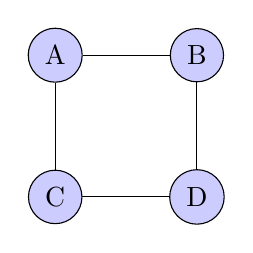
\begin{tikzpicture}[scale=0.9]
          \node[circle, draw, fill=blue!20] (A) at (0,1) {A};
          \node[circle, draw, fill=blue!20] (B) at (2,1) {B};
          \node[circle, draw, fill=blue!20] (C) at (0,-1) {C};
          \node[circle, draw, fill=blue!20] (D) at (2,-1) {D};

          \draw (A) -- (B);
          \draw (A) -- (C);
          \draw (C) -- (D);
          \draw (B) -- (D);
        \end{tikzpicture}
      \end{center}

      \textbf{Examples:}
      \begin{itemize}
        \item Friendships
        \item Two-way roads
        \item Collaborations
      \end{itemize}

      \textbf{Edge (A,B) means:}
      \begin{itemize}
        \item A can reach B
        \item B can reach A
      \end{itemize}
    \end{column}

    \begin{column}{0.5\textwidth}
      \textbf{Directed Graph:}

      Edges have direction

      \vspace{0.2cm}
      \begin{center}
        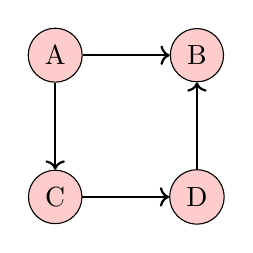
\begin{tikzpicture}[scale=0.9]
          \node[circle, draw, fill=red!20] (A) at (0,1) {A};
          \node[circle, draw, fill=red!20] (B) at (2,1) {B};
          \node[circle, draw, fill=red!20] (C) at (0,-1) {C};
          \node[circle, draw, fill=red!20] (D) at (2,-1) {D};

          \draw[->, thick] (A) -- (B);
          \draw[->, thick] (A) -- (C);
          \draw[->, thick] (C) -- (D);
          \draw[->, thick] (D) -- (B);
        \end{tikzpicture}
      \end{center}

      \textbf{Examples:}
      \begin{itemize}
        \item Twitter follows
        \item Web links
        \item Dependencies
      \end{itemize}

      \textbf{Edge A$\rightarrow$B means:}
      \begin{itemize}
        \item A can reach B
        \item B cannot reach A (unless B$\rightarrow$A)
      \end{itemize}
    \end{column}
  \end{columns}
\end{frame}

\begin{frame}[fragile]{Directed Graph Implementation}
  \begin{lstlisting}[language=Python, basicstyle=\ttfamily\small]
# Undirected: add edge in both directions
def add_undirected_edge(graph, u, v):
    graph[u].append(v)
    graph[v].append(u)

# Example: friendship network
friends = {
    'Alice': ['Bob', 'Charlie'],
    'Bob': ['Alice', 'David'],
    'Charlie': ['Alice', 'David'],
    'David': ['Bob', 'Charlie']
}

# Directed: add edge in one direction only
def add_directed_edge(graph, u, v):
    graph[u].append(v)

# Example: Twitter follows
follows = {
    'Alice': ['Bob', 'Charlie'],      # Alice follows Bob, Charlie
    'Bob': ['David'],                 # Bob follows David
    'Charlie': ['Alice', 'David'],    # Charlie follows Alice, David
    'David': []                       # David follows no one
}
  \end{lstlisting}
\end{frame}

\begin{frame}{Weighted vs Unweighted Graphs}
  \begin{columns}[T]
    \begin{column}{0.5\textwidth}
      \textbf{Unweighted Graph:}

      All edges have equal cost

      \vspace{0.2cm}
      \begin{center}
        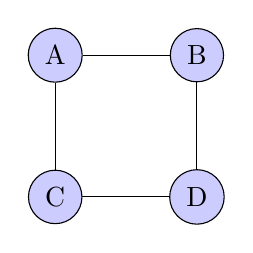
\begin{tikzpicture}[scale=0.9]
          \node[circle, draw, fill=blue!20] (A) at (0,1) {A};
          \node[circle, draw, fill=blue!20] (B) at (2,1) {B};
          \node[circle, draw, fill=blue!20] (C) at (0,-1) {C};
          \node[circle, draw, fill=blue!20] (D) at (2,-1) {D};

          \draw (A) -- (B);
          \draw (A) -- (C);
          \draw (C) -- (D);
          \draw (B) -- (D);
        \end{tikzpicture}
      \end{center}

      \textbf{Use cases:}
      \begin{itemize}
        \item Social networks
        \item Maze solving
        \item Connectivity
      \end{itemize}

      \textbf{Shortest path:}
      \begin{itemize}
        \item Use BFS
        \item Counts edges
      \end{itemize}
    \end{column}

    \begin{column}{0.5\textwidth}
      \textbf{Weighted Graph:}

      Edges have costs/weights

      \vspace{0.2cm}
      \begin{center}
        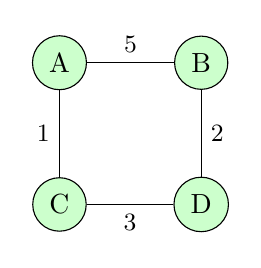
\begin{tikzpicture}[scale=0.9]
          \node[circle, draw, fill=green!20] (A) at (0,1) {A};
          \node[circle, draw, fill=green!20] (B) at (2,1) {B};
          \node[circle, draw, fill=green!20] (C) at (0,-1) {C};
          \node[circle, draw, fill=green!20] (D) at (2,-1) {D};

          \draw (A) -- node[above] {\small 5} (B);
          \draw (A) -- node[left] {\small 1} (C);
          \draw (C) -- node[below] {\small 3} (D);
          \draw (B) -- node[right] {\small 2} (D);
        \end{tikzpicture}
      \end{center}

      \textbf{Use cases:}
      \begin{itemize}
        \item Road networks
        \item Flight routes
        \item Cost optimization
      \end{itemize}

      \textbf{Shortest path:}
      \begin{itemize}
        \item Use Dijkstra's
        \item Minimizes total weight
      \end{itemize}
    \end{column}
  \end{columns}
\end{frame}

\section{Graph Traversals}

\begin{frame}{Breadth-First Search (BFS)}
  \textbf{Strategy:} Explore level by level (nearest neighbors first)

  \vspace{0.3cm}
  \textbf{Data Structure:} Queue (FIFO)

  \vspace{0.3cm}
  \begin{columns}[T]
    \begin{column}{0.45\textwidth}
      \begin{center}
        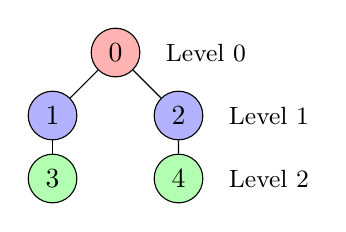
\begin{tikzpicture}[scale=0.8]
          \node[circle, draw, fill=red!30] (0) at (1,2) {0};
          \node[circle, draw, fill=blue!30] (1) at (0,1) {1};
          \node[circle, draw, fill=blue!30] (2) at (2,1) {2};
          \node[circle, draw, fill=green!30] (3) at (0,0) {3};
          \node[circle, draw, fill=green!30] (4) at (2,0) {4};

          \draw (0) -- (1);
          \draw (0) -- (2);
          \draw (1) -- (3);
          \draw (2) -- (4);

          \node[right=0.2cm of 0, draw=none] {\small Level 0};
          \node[right=0.2cm of 2, draw=none] {\small Level 1};
          \node[right=0.2cm of 4, draw=none] {\small Level 2};
        \end{tikzpicture}
      \end{center}

      \textbf{BFS from 0:} [0, 1, 2, 3, 4]
    \end{column}

    \begin{column}{0.55\textwidth}
      \textbf{Algorithm:}
      \begin{enumerate}
        \item Start at source
        \item Add to queue
        \item While queue not empty:
          \begin{itemize}
            \item Dequeue vertex
            \item Visit it
            \item Enqueue unvisited neighbors
          \end{itemize}
      \end{enumerate}

      \vspace{0.3cm}
      \textbf{Applications:}
      \begin{itemize}
        \item Shortest path (unweighted)
        \item Level-order traversal
        \item Connected components
        \item Bipartite checking
      \end{itemize}
    \end{column}
  \end{columns}

  \vspace{0.3cm}
  \textbf{Time:} O(V + E) \quad \textbf{Space:} O(V)
\end{frame}

\begin{frame}[fragile]{BFS Implementation}
  \begin{lstlisting}[language=Python, basicstyle=\ttfamily\small]
from collections import deque

def bfs(graph, start):
    visited = set([start])
    queue = deque([start])
    result = []

    while queue:
        node = queue.popleft()
        result.append(node)

        for neighbor in graph[node]:
            if neighbor not in visited:
                visited.add(neighbor)
                queue.append(neighbor)

    return result

# Example
graph = {
    0: [1, 2],
    1: [0, 3],
    2: [0, 4],
    3: [1],
    4: [2]
}
bfs(graph, 0)  # [0, 1, 2, 3, 4]
  \end{lstlisting}
\end{frame}

\begin{frame}{Depth-First Search (DFS)}
  \textbf{Strategy:} Explore as deep as possible before backtracking

  \vspace{0.3cm}
  \textbf{Data Structure:} Stack (or recursion)

  \vspace{0.3cm}
  \begin{columns}[T]
    \begin{column}{0.45\textwidth}
      \begin{center}
        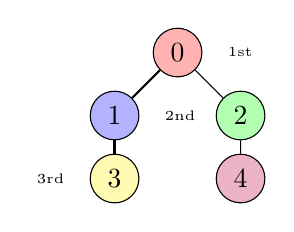
\begin{tikzpicture}[scale=0.8]
          \node[circle, draw, fill=red!30] (0) at (1,2) {0};
          \node[circle, draw, fill=blue!30] (1) at (0,1) {1};
          \node[circle, draw, fill=green!30] (2) at (2,1) {2};
          \node[circle, draw, fill=yellow!30] (3) at (0,0) {3};
          \node[circle, draw, fill=purple!30] (4) at (2,0) {4};

          \draw[thick] (0) -- (1);
          \draw (0) -- (2);
          \draw[thick] (1) -- (3);
          \draw (2) -- (4);

          \node[right=0.2cm of 0, draw=none] {\tiny 1st};
          \node[right=0.2cm of 1, draw=none] {\tiny 2nd};
          \node[left=0.2cm of 3, draw=none] {\tiny 3rd};
        \end{tikzpicture}
      \end{center}

      \textbf{DFS from 0:} [0, 1, 3, 2, 4]
    \end{column}

    \begin{column}{0.55\textwidth}
      \textbf{Algorithm:}
      \begin{enumerate}
        \item Start at source
        \item Mark as visited
        \item For each unvisited neighbor:
          \begin{itemize}
            \item Recursively DFS from it
          \end{itemize}
        \item Backtrack
      \end{enumerate}

      \vspace{0.3cm}
      \textbf{Applications:}
      \begin{itemize}
        \item Cycle detection
        \item Topological sorting
        \item Strongly connected components
        \item Path finding
        \item Maze solving
      \end{itemize}
    \end{column}
  \end{columns}

  \vspace{0.3cm}
  \textbf{Time:} O(V + E) \quad \textbf{Space:} O(V)
\end{frame}

\begin{frame}[fragile]{DFS Implementation}
  \begin{lstlisting}[language=Python, basicstyle=\ttfamily\footnotesize]
# Recursive
def dfs_recursive(graph, node, visited=None):
    if visited is None:
        visited = set()

    visited.add(node)
    result = [node]

    for neighbor in graph[node]:
        if neighbor not in visited:
            result.extend(dfs_recursive(graph, neighbor, visited))

    return result

# Iterative
def dfs_iterative(graph, start):
    visited = set()
    stack = [start]
    result = []

    while stack:
        node = stack.pop()
        if node not in visited:
            visited.add(node)
            result.append(node)

            for neighbor in reversed(graph[node]):
                if neighbor not in visited:
                    stack.append(neighbor)

    return result
  \end{lstlisting}
\end{frame}

\begin{frame}{BFS vs DFS Comparison}
  \begin{table}
    \centering
    \begin{tabular}{|l|c|c|}
      \hline
      \textbf{Feature} & \textbf{BFS} & \textbf{DFS} \\
      \hline
      Data structure & Queue & Stack/Recursion \\
      \hline
      Order & Level by level & Deep first \\
      \hline
      Shortest path & Yes (unweighted) & No \\
      \hline
      Memory & More (stores level) & Less (stores path) \\
      \hline
      Completeness & Yes & Yes (with visited) \\
      \hline
      Time & O(V + E) & O(V + E) \\
      \hline
      Space & O(V) & O(V) \\
      \hline
    \end{tabular}
  \end{table}

  \vspace{0.5cm}
  \textbf{When to use:}
  \begin{itemize}
    \item \textbf{BFS:} Shortest path, level processing, closer nodes first
    \item \textbf{DFS:} Cycle detection, topological sort, exploring all paths
  \end{itemize}
\end{frame}

\section{Connected Components and Cycles}

\begin{frame}{Connected Components}
  \textbf{Definition:} Maximal subgraphs where every pair of vertices is connected.

  \vspace{0.3cm}
  \begin{center}
    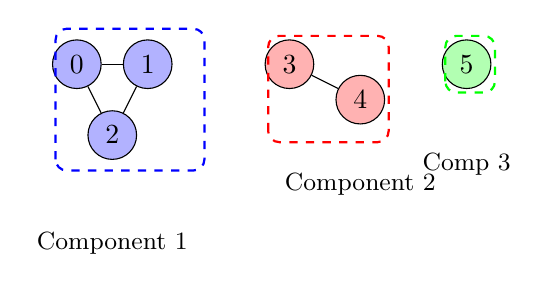
\begin{tikzpicture}[scale=0.9]
      % Component 1
      \node[circle, draw, fill=blue!30] (0) at (0,1) {0};
      \node[circle, draw, fill=blue!30] (1) at (1,1) {1};
      \node[circle, draw, fill=blue!30] (2) at (0.5,0) {2};
      \draw (0) -- (1);
      \draw (1) -- (2);
      \draw (2) -- (0);

      % Component 2
      \node[circle, draw, fill=red!30] (3) at (3,1) {3};
      \node[circle, draw, fill=red!30] (4) at (4,0.5) {4};
      \draw (3) -- (4);

      % Component 3
      \node[circle, draw, fill=green!30] (5) at (5.5,1) {5};

      \draw[dashed, blue, thick, rounded corners] (-0.3,-0.5) rectangle (1.8,1.5);
      \draw[dashed, red, thick, rounded corners] (2.7,-0.1) rectangle (4.4,1.4);
      \draw[dashed, green, thick, rounded corners] (5.2,0.6) rectangle (5.9,1.4);

      \node[below=0.8cm of 2, draw=none] {\small Component 1};
      \node[below=0.5cm of 4, draw=none] {\small Component 2};
      \node[below=0.7cm of 5, draw=none] {\small Comp 3};
    \end{tikzpicture}
  \end{center}

  \vspace{0.3cm}
  \textbf{Example:} 3 connected components: \{0,1,2\}, \{3,4\}, \{5\}

  \vspace{0.3cm}
  \textbf{Algorithm:} Run BFS/DFS from each unvisited vertex
  \begin{itemize}
    \item Each DFS/BFS finds one component
    \item Count number of DFS/BFS calls needed
  \end{itemize}
\end{frame}

\begin{frame}[fragile]{Finding Connected Components}
  \begin{lstlisting}[language=Python, basicstyle=\ttfamily\footnotesize]
def count_components(graph):
    visited = set()
    count = 0

    def dfs(node):
        visited.add(node)
        for neighbor in graph[node]:
            if neighbor not in visited:
                dfs(neighbor)

    for node in graph:
        if node not in visited:
            dfs(node)
            count += 1

    return count

def find_components(graph):
    visited = set()
    components = []

    def dfs(node, component):
        visited.add(node)
        component.append(node)
        for neighbor in graph[node]:
            if neighbor not in visited:
                dfs(neighbor, component)

    for node in graph:
        if node not in visited:
            component = []
            dfs(node, component)
            components.append(component)

    return components
  \end{lstlisting}
\end{frame}

\begin{frame}{Cycle Detection}
  \textbf{Cycle:} A path that starts and ends at the same vertex.

  \vspace{0.3cm}
  \begin{columns}[T]
    \begin{column}{0.5\textwidth}
      \textbf{Has Cycle:}
      \begin{center}
        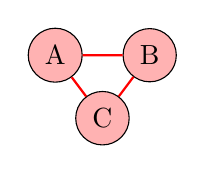
\begin{tikzpicture}[scale=0.8]
          \node[circle, draw, fill=red!30] (A) at (0,1) {A};
          \node[circle, draw, fill=red!30] (B) at (1.5,1) {B};
          \node[circle, draw, fill=red!30] (C) at (0.75,0) {C};

          \draw[thick, red] (A) -- (B);
          \draw[thick, red] (B) -- (C);
          \draw[thick, red] (C) -- (A);
        \end{tikzpicture}
      \end{center}

      Cycle: A → B → C → A
    \end{column}

    \begin{column}{0.5\textwidth}
      \textbf{No Cycle (Tree):}
      \begin{center}
        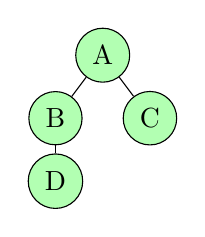
\begin{tikzpicture}[scale=0.8]
          \node[circle, draw, fill=green!30] (A) at (0.75,1.5) {A};
          \node[circle, draw, fill=green!30] (B) at (0,0.5) {B};
          \node[circle, draw, fill=green!30] (C) at (1.5,0.5) {C};
          \node[circle, draw, fill=green!30] (D) at (0,-0.5) {D};

          \draw (A) -- (B);
          \draw (A) -- (C);
          \draw (B) -- (D);
        \end{tikzpicture}
      \end{center}

      Tree: No cycles
    \end{column}
  \end{columns}

  \vspace{0.3cm}
  \textbf{Detection Methods:}
  \begin{itemize}
    \item \textbf{Undirected:} DFS with parent tracking
    \item \textbf{Directed:} DFS with color marking (White/Gray/Black)
  \end{itemize}
\end{frame}

\begin{frame}[fragile]{Cycle Detection - Undirected}
  \begin{lstlisting}[language=Python, basicstyle=\ttfamily\small]
def has_cycle_undirected(graph):
    visited = set()

    def dfs(node, parent):
        visited.add(node)

        for neighbor in graph[node]:
            if neighbor not in visited:
                if dfs(neighbor, node):
                    return True
            elif neighbor != parent:
                return True  # Back edge found (cycle)

        return False

    for node in graph:
        if node not in visited:
            if dfs(node, -1):
                return True

    return False
  \end{lstlisting}

  \vspace{0.3cm}
  \textbf{Key idea:} If we encounter a visited node that's not our parent, we found a cycle.
\end{frame}

\begin{frame}[fragile]{Cycle Detection - Directed}
  \begin{lstlisting}[language=Python, basicstyle=\ttfamily\footnotesize]
def has_cycle_directed(graph):
    WHITE, GRAY, BLACK = 0, 1, 2
    color = {node: WHITE for node in graph}

    def dfs(node):
        color[node] = GRAY  # Currently exploring

        for neighbor in graph[node]:
            if color[neighbor] == GRAY:
                return True  # Back edge (cycle)
            if color[neighbor] == WHITE and dfs(neighbor):
                return True

        color[node] = BLACK  # Finished exploring
        return False

    for node in graph:
        if color[node] == WHITE:
            if dfs(node):
                return True

    return False
  \end{lstlisting}

  \vspace{0.3cm}
  \textbf{Colors:}
  \begin{itemize}
    \item \textbf{WHITE:} Not visited
    \item \textbf{GRAY:} Currently in DFS stack (ancestor)
    \item \textbf{BLACK:} Fully explored
  \end{itemize}
\end{frame}

\section{Real-World Applications}

\begin{frame}{Social Networks}
  \textbf{Model:} Users as vertices, relationships as edges

  \vspace{0.3cm}
  \begin{center}
    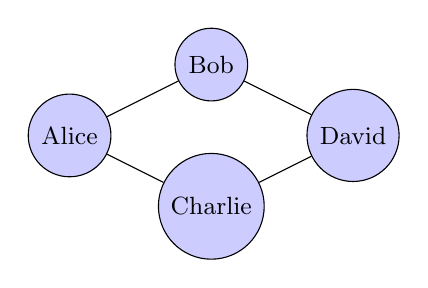
\begin{tikzpicture}[scale=0.9]
      \node[circle, draw, fill=blue!20] (alice) at (0,1) {\small Alice};
      \node[circle, draw, fill=blue!20] (bob) at (2,2) {\small Bob};
      \node[circle, draw, fill=blue!20] (charlie) at (2,0) {\small Charlie};
      \node[circle, draw, fill=blue!20] (david) at (4,1) {\small David};

      \draw (alice) -- (bob);
      \draw (alice) -- (charlie);
      \draw (bob) -- (david);
      \draw (charlie) -- (david);
    \end{tikzpicture}
  \end{center}

  \vspace{0.3cm}
  \textbf{Applications:}
  \begin{itemize}
    \item \textbf{Friend recommendations:} Friends of friends (2-hop neighbors)
    \item \textbf{Influence analysis:} Find most connected users (degree centrality)
    \item \textbf{Community detection:} Find clusters/groups
    \item \textbf{Six degrees of separation:} Shortest path between users
    \item \textbf{Viral spread:} Model information propagation
  \end{itemize}
\end{frame}

\begin{frame}[fragile]{Friend Recommendations}
  \begin{lstlisting}[language=Python, basicstyle=\ttfamily\small]
def recommend_friends(graph, user):
    """Find friends of friends"""
    friends = set(graph[user])
    recommendations = set()

    for friend in friends:
        for friend_of_friend in graph[friend]:
            if friend_of_friend != user and \
               friend_of_friend not in friends:
                recommendations.add(friend_of_friend)

    return recommendations

def find_influencers(graph, top_k=10):
    """Find most connected users (degree centrality)"""
    degrees = [(node, len(graph[node])) for node in graph]
    degrees.sort(key=lambda x: x[1], reverse=True)
    return degrees[:top_k]

# Example
friends = {
    'Alice': ['Bob', 'Charlie'],
    'Bob': ['Alice', 'David'],
    'Charlie': ['Alice', 'David'],
    'David': ['Bob', 'Charlie']
}
recommend_friends(friends, 'Alice')  # {'David'}
  \end{lstlisting}
\end{frame}

\begin{frame}{Maps and Navigation}
  \textbf{Model:} Locations as vertices, roads as weighted edges

  \vspace{0.3cm}
  \begin{center}
    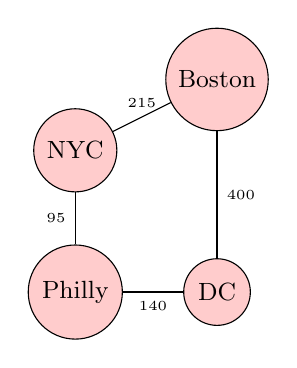
\begin{tikzpicture}[scale=0.9]
      \node[circle, draw, fill=red!20] (nyc) at (0,1) {\small NYC};
      \node[circle, draw, fill=red!20] (boston) at (2,2) {\small Boston};
      \node[circle, draw, fill=red!20] (philly) at (0,-1) {\small Philly};
      \node[circle, draw, fill=red!20] (dc) at (2,-1) {\small DC};

      \draw (nyc) -- node[above] {\tiny 215} (boston);
      \draw (nyc) -- node[left] {\tiny 95} (philly);
      \draw (philly) -- node[below] {\tiny 140} (dc);
      \draw (boston) -- node[right] {\tiny 400} (dc);
    \end{tikzpicture}
  \end{center}

  \vspace{0.3cm}
  \textbf{Applications:}
  \begin{itemize}
    \item \textbf{Route planning:} Shortest path (Dijkstra's, A*)
    \item \textbf{Traffic optimization:} Alternative routes, congestion avoidance
    \item \textbf{Delivery routing:} Traveling salesman problem (TSP)
    \item \textbf{Public transit:} Multi-modal routing (bus + train + walk)
    \item \textbf{Ride sharing:} Match drivers with passengers
  \end{itemize}
\end{frame}

\begin{frame}{Web and Internet}
  \textbf{Model:} Pages/routers as vertices, links/connections as edges

  \vspace{0.3cm}
  \begin{center}
    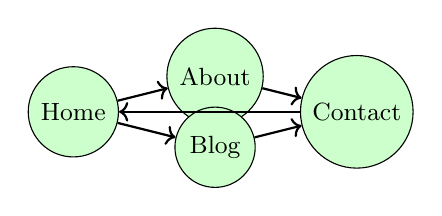
\begin{tikzpicture}[scale=0.9]
      \node[circle, draw, fill=green!20] (home) at (0,1) {\small Home};
      \node[circle, draw, fill=green!20] (about) at (2,1.5) {\small About};
      \node[circle, draw, fill=green!20] (blog) at (2,0.5) {\small Blog};
      \node[circle, draw, fill=green!20] (contact) at (4,1) {\small Contact};

      \draw[->, thick] (home) -- (about);
      \draw[->, thick] (home) -- (blog);
      \draw[->, thick] (about) -- (contact);
      \draw[->, thick] (blog) -- (contact);
      \draw[->, thick] (contact) -- (home);
    \end{tikzpicture}
  \end{center}

  \vspace{0.3cm}
  \textbf{Applications:}
  \begin{itemize}
    \item \textbf{PageRank:} Rank web pages by importance/authority
    \item \textbf{Web crawling:} BFS/DFS to discover new pages
    \item \textbf{Network routing:} Find optimal packet paths
    \item \textbf{Load balancing:} Distribute traffic across servers
    \item \textbf{Link analysis:} Detect spam, find related pages
  \end{itemize}
\end{frame}

\begin{frame}{Other Applications}
  \textbf{Dependency Graphs:}
  \begin{itemize}
    \item Build systems: Compile order (topological sort)
    \item Package managers: Install dependencies
    \item Task scheduling: Prerequisite handling
  \end{itemize}

  \vspace{0.3cm}
  \textbf{Recommendation Systems:}
  \begin{itemize}
    \item User-item bipartite graphs
    \item Collaborative filtering
    \item Content-based recommendations
  \end{itemize}

  \vspace{0.3cm}
  \textbf{Science and Research:}
  \begin{itemize}
    \item Biology: Protein interaction networks, phylogenetic trees
    \item Chemistry: Molecular structures, reaction networks
    \item Physics: Particle interactions
    \item Social science: Citation networks, collaboration graphs
  \end{itemize}

  \vspace{0.3cm}
  \textbf{Games and AI:}
  \begin{itemize}
    \item Pathfinding: A* algorithm in games
    \item State space search: Game trees, puzzle solving
  \end{itemize}
\end{frame}

\section{Complexity Analysis}

\begin{frame}{Time Complexity Summary}
  \begin{table}
    \centering
    \small
    \begin{tabular}{|l|c|c|}
      \hline
      \textbf{Operation} & \textbf{Adjacency List} & \textbf{Adjacency Matrix} \\
      \hline
      Add vertex & O(1) & O(V$^2$) (resize) \\
      \hline
      Add edge & O(1) & O(1) \\
      \hline
      Remove vertex & O(E) & O(V$^2$) \\
      \hline
      Remove edge & O(E) & O(1) \\
      \hline
      Check edge & O(degree) & O(1) \\
      \hline
      Get neighbors & O(degree) & O(V) \\
      \hline
      BFS/DFS & O(V + E) & O(V$^2$) \\
      \hline
      Dijkstra & O((V+E) log V) & O(V$^2$) \\
      \hline
    \end{tabular}
  \end{table}

  \vspace{0.3cm}
  \textbf{Key insight:}
  \begin{itemize}
    \item Adjacency list better for sparse graphs (E $\ll$ V$^2$)
    \item Adjacency matrix better for dense graphs (E $\approx$ V$^2$)
  \end{itemize}
\end{frame}

\begin{frame}{Space Complexity}
  \begin{table}
    \centering
    \begin{tabular}{|l|c|c|}
      \hline
      \textbf{Representation} & \textbf{Space} & \textbf{Best For} \\
      \hline
      Adjacency List & O(V + E) & Sparse graphs \\
      \hline
      Adjacency Matrix & O(V$^2$) & Dense graphs \\
      \hline
      Edge List & O(E) & Simple storage \\
      \hline
    \end{tabular}
  \end{table}

  \vspace{0.5cm}
  \textbf{Graph Density:}
  \begin{itemize}
    \item \textbf{Sparse:} E = O(V), few edges
      \begin{itemize}
        \item Example: Social networks (avg degree $\sim$100)
        \item Use adjacency list
      \end{itemize}
    \item \textbf{Dense:} E = O(V$^2$), many edges
      \begin{itemize}
        \item Example: Complete graph (all pairs connected)
        \item Use adjacency matrix
      \end{itemize}
  \end{itemize}
\end{frame}

\begin{frame}{Memory Calculations}
  \textbf{Example: 1 million vertices}

  \vspace{0.3cm}
  \textbf{Sparse graph (avg degree = 10):}
  \begin{itemize}
    \item E $\approx$ 5 million edges
    \item Adjacency list: (V + E) $\times$ 8 bytes = 40 MB
    \item Adjacency matrix: V $\times$ V $\times$ 1 byte = 1 TB (impractical!)
  \end{itemize}

  \vspace{0.3cm}
  \textbf{Dense graph (E = V$^2$/2):}
  \begin{itemize}
    \item E $\approx$ 500 billion edges
    \item Adjacency list: (V + E) $\times$ 8 bytes = 4 TB
    \item Adjacency matrix: V $\times$ V $\times$ 1 byte = 1 TB (better!)
  \end{itemize}

  \vspace{0.3cm}
  \textbf{Practical considerations:}
  \begin{itemize}
    \item Small graphs (V $<$ 1000): Either works
    \item Medium graphs (V $<$ 100K): Adjacency list usually better
    \item Large graphs (V $>$ 1M): Must use adjacency list
    \item Very dense: Consider compressed formats
  \end{itemize}
\end{frame}

\section{Summary}

\begin{frame}{Key Concepts Recap}
  \textbf{Graph Fundamentals:}
  \begin{itemize}
    \item Graph G = (V, E): vertices and edges
    \item Models relationships between entities
    \item Directed vs undirected, weighted vs unweighted
  \end{itemize}

  \vspace{0.3cm}
  \textbf{Representations:}
  \begin{itemize}
    \item \textbf{Adjacency list:} O(V + E) space, best for sparse
    \item \textbf{Adjacency matrix:} O(V$^2$) space, best for dense
  \end{itemize}

  \vspace{0.3cm}
  \textbf{Traversals:}
  \begin{itemize}
    \item \textbf{BFS:} Level by level, shortest path (unweighted)
    \item \textbf{DFS:} Deep first, cycle detection, topological sort
  \end{itemize}

  \vspace{0.3cm}
  \textbf{Analysis:}
  \begin{itemize}
    \item Connected components: Find separate subgraphs
    \item Cycle detection: Identify circular dependencies
    \item Both use BFS/DFS: O(V + E)
  \end{itemize}
\end{frame}

\begin{frame}{Applications Recap}
  \textbf{Major Use Cases:}
  \begin{itemize}
    \item \textbf{Social networks:} Friend recommendations, influence analysis
    \item \textbf{Maps/navigation:} Route planning, traffic optimization
    \item \textbf{Web:} PageRank, web crawling, network routing
    \item \textbf{Dependencies:} Build systems, package managers
    \item \textbf{Science:} Biology, chemistry, physics networks
  \end{itemize}

  \vspace{0.3cm}
  \textbf{Common Algorithms:}
  \begin{itemize}
    \item BFS, DFS: O(V + E)
    \item Dijkstra's shortest path: O((V+E) log V)
    \item Topological sort: O(V + E)
    \item Connected components: O(V + E)
    \item Cycle detection: O(V + E)
  \end{itemize}
\end{frame}

\begin{frame}{Practice Problems}
  \textbf{Basic:}
  \begin{itemize}
    \item Implement adjacency list and matrix representations
    \item Implement BFS and DFS
    \item Count connected components
    \item Detect cycles in undirected graph
  \end{itemize}

  \vspace{0.3cm}
  \textbf{Intermediate:}
  \begin{itemize}
    \item Find shortest path in unweighted graph (BFS)
    \item Check if graph is bipartite
    \item Find all paths from source to destination
    \item Detect cycles in directed graph
    \item Clone a graph
  \end{itemize}

  \vspace{0.3cm}
  \textbf{Advanced:}
  \begin{itemize}
    \item Implement Dijkstra's algorithm
    \item Topological sort (course schedule problems)
    \item Strongly connected components (Kosaraju's/Tarjan's)
    \item Minimum spanning tree (Prim's/Kruskal's)
    \item Network flow problems
  \end{itemize}
\end{frame}

\begin{frame}{Implementation Tips}
  \textbf{Best Practices:}
  \begin{itemize}
    \item Use adjacency list for most problems
    \item Always track visited nodes in BFS/DFS
    \item Handle disconnected graphs (multiple components)
    \item Consider edge cases: empty graph, single vertex, cycles
  \end{itemize}

  \vspace{0.3cm}
  \textbf{Common Pitfalls:}
  \begin{itemize}
    \item Forgetting to mark nodes as visited (infinite loops)
    \item Not handling directed vs undirected correctly
    \item Using wrong algorithm (BFS for shortest weighted path)
    \item Memory issues with large dense graphs
  \end{itemize}

  \vspace{0.3cm}
  \textbf{Optimization:}
  \begin{itemize}
    \item Use sets for O(1) visited checks
    \item Use deque for BFS (efficient popleft)
    \item Consider Union-Find for connectivity problems
    \item Profile before optimizing representation
  \end{itemize}
\end{frame}

\begin{frame}{Further Learning}
  \textbf{Advanced Topics:}
  \begin{itemize}
    \item \textbf{Shortest paths:} Dijkstra's, Bellman-Ford, Floyd-Warshall, A*
    \item \textbf{Minimum spanning trees:} Prim's, Kruskal's
    \item \textbf{Network flow:} Ford-Fulkerson, max flow min cut
    \item \textbf{Strongly connected components:} Kosaraju's, Tarjan's
    \item \textbf{Graph coloring:} Chromatic number, map coloring
  \end{itemize}

  \vspace{0.3cm}
  \textbf{Resources:}
  \begin{itemize}
    \item Practice on LeetCode graph problems
    \item Study graph algorithms in CLRS textbook
    \item Visualize with tools: Graphviz, NetworkX
    \item Build real projects: social network, route planner
  \end{itemize}

  \vspace{0.3cm}
  \textbf{Projects:}
  \begin{itemize}
    \item Implement social network with friend recommendations
    \item Build shortest path finder for maps
    \item Create web crawler using BFS
    \item Design package dependency resolver
  \end{itemize}
\end{frame}

\begin{frame}
  \begin{center}
    {\Huge Thank You!}

    \vspace{1cm}
    {\Large Questions?}

    \vspace{1cm}
    \textbf{Graphs: Connecting the World Through Data}
  \end{center}
\end{frame}

\end{document}
